%\documentclass{beamer}

\documentclass[handout]{beamer}
 
\usepackage[utf8]{inputenc}
\usepackage{graphicx}
\usepackage{wrapfig}
\usepackage{lipsum}
\usepackage{hyperref}
\usepackage{tabularx}
\usepackage{amsmath}
\usepackage{enumerate}
\usepackage[utf8]{inputenc}
\usepackage{tikz}
\usepackage{circuitikz}

\usepackage{pgfpages}

%\mode<handout>{%
%    \pgfpagesuselayout{4 on 1}[letter] 
%    \setbeameroption{show notes}
%}

\renewcommand{\vec}[1]{\mathbf{#1}} % Display vectors as boldface %

\let\oldhat\hat   % Also display hats as boldface
\renewcommand{\hat}[1]{\oldhat{\mathbf{#1}}} % Also display hats as boldface
 
%Information to be included in the title page:
\title{Physics 231}
\subtitle{Lecture 2: Resistor Circuits}
\author{Eric Landahl}
\institute{DePaul University Physics Department}
 
\begin{document}
 
\frame{\titlepage}

\begin{frame}
\frametitle{Table of Contents}
\tableofcontents
\end{frame}

\maketitle

\section{Single Resistor Circuit}

\subsection{}

\begin{frame}{\secname : \subsecname}

\begin{figure}
\begin{tikzpicture}

 \draw (2,10.5) to[short,-o] (1,10.5); % Connect to 5 V DC
 \draw (1,10.5) node[anchor=east] {V$_{in}$};
 
% Comment one of the two following lines
%\draw (2,10.5) to[ammeter,color=gray] (4,10.5); % Show ammeter 
\draw (2,10.5) to[short] (4,10.5); % or connect with short
  
 \draw  (4,10.5) to[R=$R_1$] (4,8);
 \draw (2,8) to[short,-o] (1,8); % Connect to 0 V DC
  
% Comment one of the two following lines
%\draw (2,8) to[ammeter,color=gray] (4,8); % Show lower ammeter 
 \draw (2,8) to[short] (4,8); % or connect with short
  
 \draw (1,8) node[anchor=east] {0 V};
 
% Add optional volt meter
%  \draw [gray] (4,10.5) -- (6,10.5);
%  \draw [gray] (4,8) -- (6,8);
%  \draw (6,10.5) to[voltmeter,color=gray] (6,8);

\end{tikzpicture}
\end{figure} 

\begin{equation}
    V=IR
\end{equation}

\begin{equation}
    P=IV
\end{equation}

%\vspace{0.5 cm}
%
%\noindent
%
%Questions:
%\begin{enumerate}
%    \item Write $P$ in terms of $V$ and $R$ only.
%    \item Write $P$ in terms of $I$ and $R$ only.
%    \item Determine the power in an example circuit.
%    \item Compare the power in your circuit to other examples of power.
%\end{enumerate}

\end{frame}

\subsection{Measuring Voltage}

\begin{frame}{\secname : \subsecname}

\begin{figure}
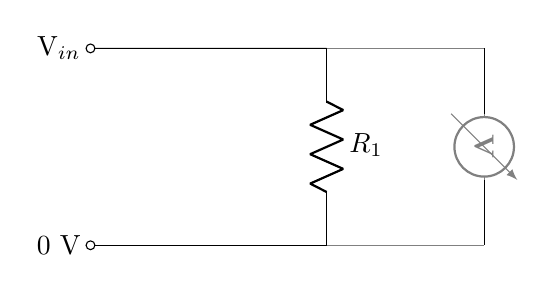
\begin{tikzpicture}

 \draw (2,10.5) to[short,-o] (1,10.5); % Connect to 5 V DC
 \draw (1,10.5) node[anchor=east] {V$_{in}$};
 
% Comment one of the two following lines
%\draw (2,10.5) to[ammeter,color=gray] (4,10.5); % Show ammeter 
\draw (2,10.5) to[short] (4,10.5); % or connect with short
  
 \draw  (4,10.5) to[R=$R_1$] (4,8);
 \draw (2,8) to[short,-o] (1,8); % Connect to 0 V DC
  
% Comment one of the two following lines
%\draw (2,8) to[ammeter,color=gray] (4,8); % Show lower ammeter 
 \draw (2,8) to[short] (4,8); % or connect with short
  
 \draw (1,8) node[anchor=east] {0 V};
 
% Add optional volt meter
  \draw [gray] (4,10.5) -- (6,10.5);
  \draw [gray] (4,8) -- (6,8);
  \draw (6,10.5) to[voltmeter,color=gray] (6,8);

\end{tikzpicture}
\end{figure} 

\end{frame}

\subsection{Measuring Current}

\begin{frame}{\secname : \subsecname}

\begin{figure}
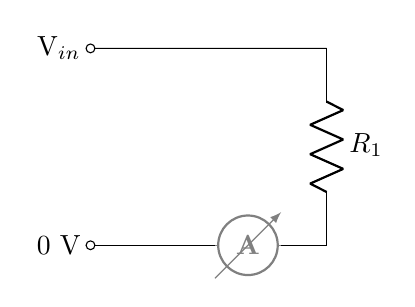
\begin{tikzpicture}

 \draw (2,10.5) to[short,-o] (1,10.5); % Connect to 5 V DC
 \draw (1,10.5) node[anchor=east] {V$_{in}$};
 
% Comment one of the two following lines
%\draw (2,10.5) to[ammeter,color=gray] (4,10.5); % Show ammeter 
\draw (2,10.5) to[short] (4,10.5); % or connect with short
  
 \draw  (4,10.5) to[R=$R_1$] (4,8);
 \draw (2,8) to[short,-o] (1,8); % Connect to 0 V DC
  
% Comment one of the two following lines
\draw (2,8) to[ammeter,color=gray] (4,8); % Show lower ammeter 
% \draw (2,8) to[short] (4,8); % or connect with short
  
 \draw (1,8) node[anchor=east] {0 V};
 
% Add optional volt meter
%  \draw [gray] (4,10.5) -- (6,10.5);
%  \draw [gray] (4,8) -- (6,8);
%  \draw (6,10.5) to[voltmeter,color=gray] (6,8);

\end{tikzpicture}
\end{figure} 

\center{or}


\begin{figure}
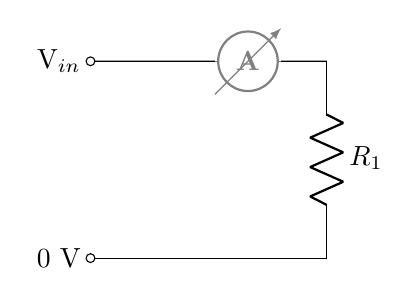
\begin{tikzpicture}

 \draw (2,10.5) to[short,-o] (1,10.5); % Connect to 5 V DC
 \draw (1,10.5) node[anchor=east] {V$_{in}$};
 
% Comment one of the two following lines
\draw (2,10.5) to[ammeter,color=gray] (4,10.5); % Show ammeter 
%\draw (2,10.5) to[short] (4,10.5); % or connect with short
  
 \draw  (4,10.5) to[R=$R_1$] (4,8);
 \draw (2,8) to[short,-o] (1,8); % Connect to 0 V DC
  
% Comment one of the two following lines
% \draw (2,8) to[ammeter,color=gray] (4,8); % Show lower ammeter 
\draw (2,8) to[short] (4,8); % or connect with short
  
 \draw (1,8) node[anchor=east] {0 V};
 
% Add optional volt meter
%  \draw [gray] (4,10.5) -- (6,10.5);
%  \draw [gray] (4,8) -- (6,8);
%  \draw (6,10.5) to[voltmeter,color=gray] (6,8);

\end{tikzpicture}
\end{figure} 

\end{frame}

\subsection{Measuring Voltage and Current}

\begin{frame}{\secname : \subsecname}

\begin{figure}
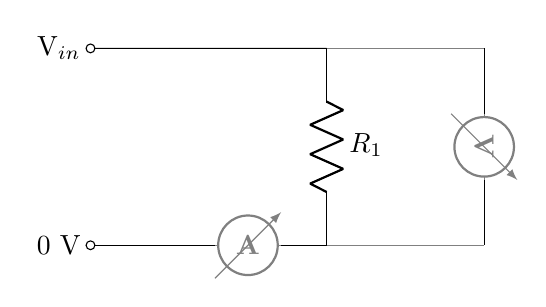
\begin{tikzpicture}

 \draw (2,10.5) to[short,-o] (1,10.5); % Connect to 5 V DC
 \draw (1,10.5) node[anchor=east] {V$_{in}$};
 
% Comment one of the two following lines
%\draw (2,10.5) to[ammeter,color=gray] (4,10.5); % Show ammeter 
\draw (2,10.5) to[short] (4,10.5); % or connect with short
  
 \draw  (4,10.5) to[R=$R_1$] (4,8);
 \draw (2,8) to[short,-o] (1,8); % Connect to 0 V DC
  
% Comment one of the two following lines
 \draw (2,8) to[ammeter,color=gray] (4,8); % Show lower ammeter 
% \draw (2,8) to[short] (4,8); % or connect with short
  
 \draw (1,8) node[anchor=east] {0 V};
 
% Add optional volt meter
  \draw [gray] (4,10.5) -- (6,10.5);
  \draw [gray] (4,8) -- (6,8);
  \draw (6,10.5) to[voltmeter,color=gray] (6,8);

\end{tikzpicture}
\end{figure} 

\end{frame}

\section{Equivalent Resistor Circuits}
\subsection{Resistors in Series}

\begin{frame}{\secname : \subsecname}
\begin{figure}
\begin{tikzpicture}

 \draw (4,10.5) to[short,-o] (1,10.5); % Connect to 5 V DC
 \draw (1,10.5) node[anchor=east] {V$_{in}$};
 \draw  (4,10.5) to[R=$R_1$] (4,8);
 \draw (4,8) to[R=$R_2$] (4,5.5);
 \draw (4,5.5) to[short,-o] (1,5.5); % Connect to 5 V DC
 \draw (1,5.5) node[anchor=east] {0 V};

\end{tikzpicture}
\end{figure}

\end{frame}
\begin{frame}{\secname : \subsecname}

1. Convert a more complicated arrangement or resistors into a simpler arrangement for easier calculations.  

\begin{equation}
    R_{eq}=R_1+R_2
\end{equation}

\begin{equation}
    I = \dfrac{V_{in}}{R_{eq}}
\end{equation}

\begin{figure}
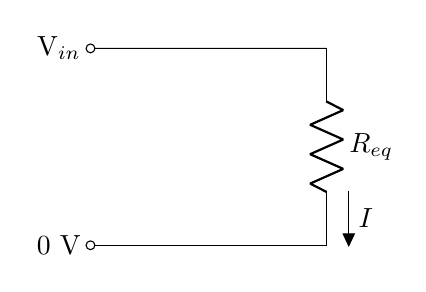
\begin{tikzpicture}

 \draw (2,10.5) to[short,-o] (1,10.5); % Connect to 5 V DC
 \draw (1,10.5) node[anchor=east] {V$_{in}$};
 
% Comment one of the two following lines
%\draw (2,10.5) to[ammeter,color=gray] (4,10.5); % Show ammeter 
\draw (2,10.5) to[short] (4,10.5); % or connect with short
  
 \draw  (4,10.5) to[R=$R_{eq}$, f^>=$I$] (4,8);
 \draw (2,8) to[short,-o] (1,8); % Connect to 0 V DC
  
% Comment one of the two following lines
%\draw (2,8) to[ammeter,color=gray] (4,8); % Show lower ammeter 
 \draw (2,8) to[short] (4,8); % or connect with short
  
 \draw (1,8) node[anchor=east] {0 V};
 
% Add optional volt meter
%  \draw [gray] (4,10.5) -- (6,10.5);
%  \draw [gray] (4,8) -- (6,8);
%  \draw (6,10.5) to[voltmeter,color=gray] (6,8);

\end{tikzpicture}
\end{figure} 

\end{frame}

\begin{frame}{\secname : \subsecname}

2. Apply these results to the more complex configuration.

\begin{equation}
    V_1 = IR_1 = \left( \dfrac{V_{in}}{R_{eq}} \right) R_1 =  \dfrac{R_1}{R_1+R_2} V_{in}
\end{equation}

\begin{equation}
    V_2 = IR_2 = \left( \dfrac{V_{in}}{R_{eq}} \right) R_2 =  \dfrac{R_2}{R_1+R_2} V_{in}
\end{equation}

\begin{figure}[b!]
\begin{tikzpicture}
 \draw (4,4.5) to[short,-o] (1,4.5); % Connect to 5 V DC
 \draw (1,4.5) node[anchor=northeast] {V$_{in}$};
 \draw  (4,4.5) to[R=$R_1$, v_>=$V_1$] (4,2.5);
 \draw (4,2.5) to[R=$R_2$, f^>=$I$, v_>=$V_2$] (4,0.25);
 \draw (4,0.25) to[short,-o] (1,0.25); % Connect to 5 V DC
 \draw (1,0.25) node[anchor=southeast] {0 V};
\end{tikzpicture}
\end{figure}
\end{frame}

\subsection{Resistors in Parallel}

\begin{frame}{\secname : \subsecname}

The voltage is the same across both resistors, but each has a different current.

\vspace{0.5 cm}

\begin{figure}
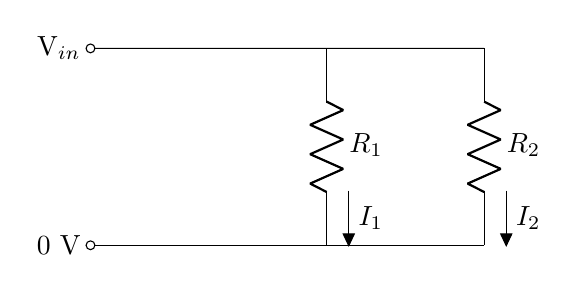
\begin{tikzpicture}

 \draw (2,10.5) to[short,-o] (1,10.5); % Connect to 5 V DC
 \draw (1,10.5) node[anchor=east] {V$_{in}$};
 
% Comment one of the two following lines
%\draw (2,10.5) to[ammeter,color=gray] (4,10.5); % Show ammeter 
\draw (2,10.5) to[short] (4,10.5); % or connect with short
  
 \draw  (4,10.5) to[R=$R_1$, f^>=$I_1$,] (4,8);
 \draw (2,8) to[short,-o] (1,8); % Connect to 0 V DC
 
 \draw (4,10.5) to[short] (6,10.5);
 \draw (6,10.5) to[R=$R_2$, f^>=$I_2$,] (6,8);
 \draw (6,8) to[short] (4,8);
  
% Comment one of the two following lines
%\draw (2,8) to[ammeter,color=gray] (4,8); % Show lower ammeter 
 \draw (2,8) to[short] (4,8); % or connect with short
  
 \draw (1,8) node[anchor=east] {0 V};
 
% Add optional volt meter
%  \draw [gray] (4,10.5) -- (6,10.5);
%  \draw [gray] (4,8) -- (6,8);
%  \draw (6,10.5) to[voltmeter,color=gray] (6,8);

\end{tikzpicture}
\end{figure} 
\end{frame}


\begin{frame}{\secname : \subsecname}
Convert the parallel resistor configuration into a single equivalent resistor.

    \begin{figure}

\begin{equation}
    \dfrac{1}{R_{eq}} = \dfrac{1}{R_1} + \dfrac{1}{R_2}
\end{equation}

\vspace{0.5 cm}
    
\begin{tikzpicture}

 \draw (2,10.5) to[short,-o] (1,10.5); % Connect to 5 V DC
 \draw (1,10.5) node[anchor=east] {V$_{in}$};
 
% Comment one of the two following lines
%\draw (2,10.5) to[ammeter,color=gray] (4,10.5); % Show ammeter 
\draw (2,10.5) to[short] (4,10.5); % or connect with short
  
 \draw  (4,10.5) to[R=$R_{eq}$] (4,8);
 \draw (2,8) to[short,-o] (1,8); % Connect to 0 V DC
  
% Comment one of the two following lines
%\draw (2,8) to[ammeter,color=gray] (4,8); % Show lower ammeter 
 \draw (2,8) to[short] (4,8); % or connect with short
  
 \draw (1,8) node[anchor=east] {0 V};
 
% Add optional volt meter
%  \draw [gray] (4,10.5) -- (6,10.5);
%  \draw [gray] (4,8) -- (6,8);
%  \draw (6,10.5) to[voltmeter,color=gray] (6,8);

\end{tikzpicture}
\end{figure} 
\end{frame}

\begin{frame}{\secname : \subsecname}

Calculate the current through the entire circuit.

\begin{equation}
    I = \dfrac{V_{in}}{R_{eq}} = V_{in} \left( \dfrac{1}{R_1} + \dfrac{1}{R_2} \right)
\end{equation}

\vspace{0.5 cm}

\begin{figure}
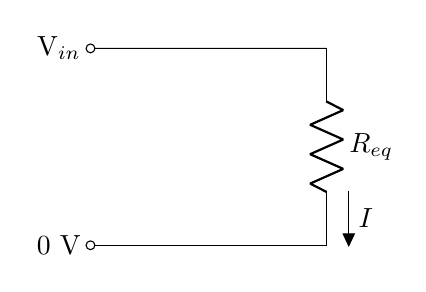
\begin{tikzpicture}

 \draw (2,10.5) to[short,-o] (1,10.5); % Connect to 5 V DC
 \draw (1,10.5) node[anchor=east] {V$_{in}$};
 
% Comment one of the two following lines
%\draw (2,10.5) to[ammeter,color=gray] (4,10.5); % Show ammeter 
\draw (2,10.5) to[short] (4,10.5); % or connect with short
  
 \draw  (4,10.5) to[R=$R_{eq}$, f^=$I$] (4,8);
 \draw (2,8) to[short,-o] (1,8); % Connect to 0 V DC
  
% Comment one of the two following lines
%\draw (2,8) to[ammeter,color=gray] (4,8); % Show lower ammeter 
 \draw (2,8) to[short] (4,8); % or connect with short
  
 \draw (1,8) node[anchor=east] {0 V};
 
% Add optional volt meter
%  \draw [gray] (4,10.5) -- (6,10.5);
%  \draw [gray] (4,8) -- (6,8);
%  \draw (6,10.5) to[voltmeter,color=gray] (6,8);

\end{tikzpicture}
\end{figure} 
\end{frame}


\begin{frame}{\secname : \subsecname}

Use the fact that all voltages are the same to calculate the current through each resistor.

\begin{equation}
    V_{in} = I_1 R_1 = I_2 R_2 = I R_{eq}
\end{equation}

and therefore

\begin{equation}
    I_1 = I \dfrac{R_{eq}}{R_1} = \dfrac{V_1}{R_1}, \quad I_2 = I \dfrac{R_{eq}}{R_2} = \dfrac{V_2}{R_2}
\end{equation}

\vspace{0.5 cm}

\begin{figure}
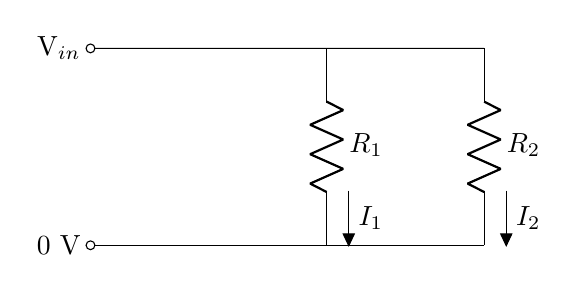
\begin{tikzpicture}

 \draw (2,10.5) to[short,-o] (1,10.5); % Connect to 5 V DC
 \draw (1,10.5) node[anchor=east] {V$_{in}$};
 
% Comment one of the two following lines
%\draw (2,10.5) to[ammeter,color=gray] (4,10.5); % Show ammeter 
\draw (2,10.5) to[short] (4,10.5); % or connect with short
  
 \draw  (4,10.5) to[R=$R_1$, f^>=$I_1$,] (4,8);
 \draw (2,8) to[short,-o] (1,8); % Connect to 0 V DC
 
 \draw (4,10.5) to[short] (6,10.5);
 \draw (6,10.5) to[R=$R_2$, f^>=$I_2$,] (6,8);
 \draw (6,8) to[short] (4,8);
  
% Comment one of the two following lines
%\draw (2,8) to[ammeter,color=gray] (4,8); % Show lower ammeter 
 \draw (2,8) to[short] (4,8); % or connect with short
  
 \draw (1,8) node[anchor=east] {0 V};
 
% Add optional volt meter
%  \draw [gray] (4,10.5) -- (6,10.5);
%  \draw [gray] (4,8) -- (6,8);
%  \draw (6,10.5) to[voltmeter,color=gray] (6,8);

\end{tikzpicture}
\end{figure} 

Verify that the currents add up: $I = I_1 + I_2$.

\end{frame}

\subsection{Loaded Voltage Divider}

\begin{frame}{\secname : \subsecname}
Goal: Determine current and voltage (and power dissipation) through each resistor with and without the load resistor connected.
\begin{figure}
\begin{tikzpicture}

% Gray backgorund box (can be commented out)
% \draw [fill=gray] (0,4.5) rectangle (5,11.5);

 \draw (4,10.5) to[short,-o] (1,10.5); % Connect to 5 V DC
 \draw (1,10.5) node[anchor=east] {V$_{in}$};
 \draw  (4,10.5) to[R=$R_1$] (4,8);
 \draw (6,8) node[anchor=west] {V$_{out}$};
 \draw (4,8) to[short,-o] (6,8);
 \draw (4,8) to[R=$R_2$] (4,5.5);
 \draw (4,5.5) to[short,-o] (1,5.5); 
 \draw (1,5.5) node[anchor=east] {0 V};
 \draw (4,5.5) to[short,-o] (6,5.5);
 \draw (6,5.5) node[anchor=west] {0 V};
 
% Load resistor (can be commented out)
 \draw [dash dot] (7,5.5) to[short](8,5.5);
 \draw [dash dot] (7,8) to[short](8,8);
 \draw (8,8) to[R=$R_{Load}$] (8,5.5);

\end{tikzpicture}
\end{figure}

\end{frame}

\begin{frame}{\secname : \subsecname}
Case I:  Unloaded (refer back to Resistors in Series)

\begin{figure}
\begin{tikzpicture}

 \draw (4,10.5) to[short,-o] (1,10.5); % Connect to 5 V DC
 \draw (1,10.5) node[anchor=east] {V$_{in}$};
 % \draw (4,10.5) to[short,-o] (6,10.5);
 \draw  (4,10.5) to[R=$R_1$] (4,8);
 \draw (4,8) to[short,-o] (6,8);
 \draw (4,8) to[R=$R_2$] (4,5.5);
 \draw (4,5.5) to[short,-o] (6,5.5);
 %\draw (6,8) to[R=$R_{Load}$] (6,5.5);
  \draw (4,5.5) to[short,-o] (1,5.5); % Connect to 5 V DC
 \draw (1,5.5) node[anchor=east] {0 V};

\end{tikzpicture}
\end{figure}

\end{frame}

\begin{frame}{\secname : \subsecname}
Case II:  Loaded (refer back to Resistors in Parallel, \emph{then} Resistors in Series)

\begin{figure}
\begin{tikzpicture}

 \draw (4,10.5) to[short,-o] (1,10.5); % Connect to 5 V DC
 \draw (1,10.5) node[anchor=east] {V$_{in}$};
 % \draw (4,10.5) to[short,-o] (6,10.5);
 \draw  (4,10.5) to[R=$R_1$] (4,8);
 \draw (4,8) to[short,-o] (6,8);
 \draw (4,8) to[R=$R_2$] (4,5.5);
 \draw (4,5.5) to[short,-o] (6,5.5);
 \draw (6,8) to[R=$R_{Load}$] (6,5.5);
  \draw (4,5.5) to[short,-o] (1,5.5); % Connect to 5 V DC
 \draw (1,5.5) node[anchor=east] {0 V};

\end{tikzpicture}
\end{figure}

\end{frame}

\section{Equivalent Circuits}
\subsection{Voltage Divider}

\begin{frame}{\secname : \subsecname}
Replace the entire source with a "black box" with an equivalent voltage and an equivalent resistance in series.
\begin{figure}
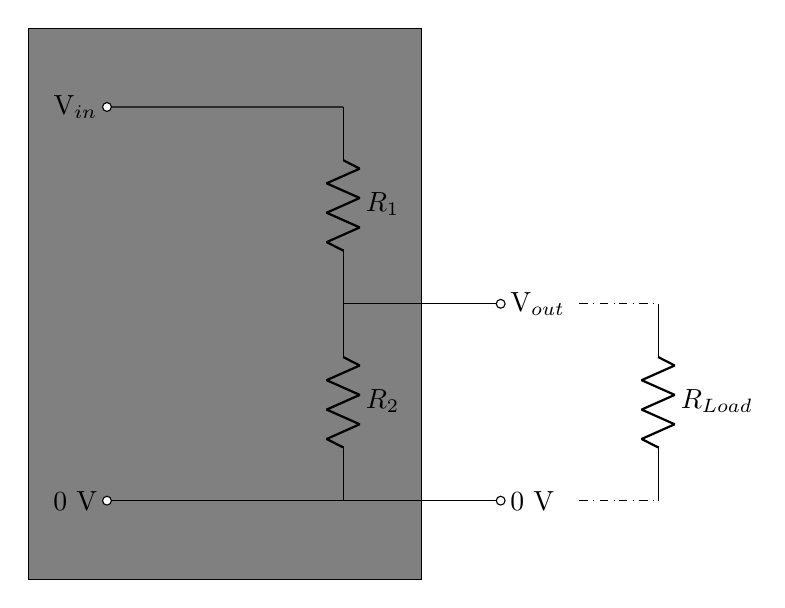
\begin{tikzpicture}

% Gray backgorund box (can be commented out)
\draw [fill=gray] (0,4.5) rectangle (5,11.5);

 \draw (4,10.5) to[short,-o] (1,10.5); % Connect to 5 V DC
 \draw (1,10.5) node[anchor=east] {V$_{in}$};
 \draw  (4,10.5) to[R=$R_1$] (4,8);
 \draw (6,8) node[anchor=west] {V$_{out}$};
 \draw (4,8) to[short,-o] (6,8);
 \draw (4,8) to[R=$R_2$] (4,5.5);
 \draw (4,5.5) to[short,-o] (1,5.5); 
 \draw (1,5.5) node[anchor=east] {0 V};
 \draw (4,5.5) to[short,-o] (6,5.5);
 \draw (6,5.5) node[anchor=west] {0 V};
 
% Load resistor (can be commented out)
 \draw [dash dot] (7,5.5) to[short](8,5.5);
 \draw [dash dot] (7,8) to[short](8,8);
 \draw (8,8) to[R=$R_{Load}$] (8,5.5);

\end{tikzpicture}
\end{figure}

\end{frame}


\begin{frame}{\secname : \subsecname}
The ``Thevenin Equivalent'' Circuit is defined to be the one where the output voltage $V_{out}=\frac{V_{th}}{2}$  when connected to a load $R_{Load}=R_{th}$.  \emph{Every power supply has a $V_{th}$ and $R_{th}$.}
\begin{figure}
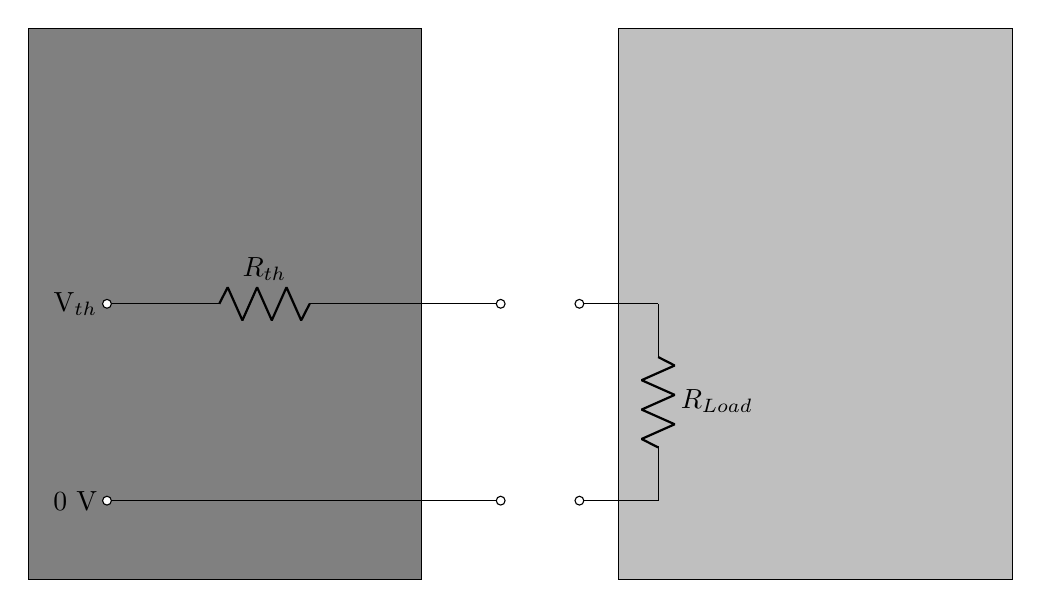
\begin{tikzpicture}

% Source
% Gray backgorund box (can be commented out)
\draw [fill=gray] (0,4.5) rectangle (5,11.5);

 \draw (2,8) to [short,-o] (1,8);
 \draw (2,8) to[R=$R_{th}$] (4,8); % Connect to 5 V DC
 \draw (1,8) node[anchor=east] {V$_{th}$};
 %\draw  (4,10.5) to[R=$R_{th}$] (4,8);
 %\draw (6,8) node[anchor=west] {V$_{th}$};
 \draw (4,8) to[short,-o] (6,8);
 % \draw (4,8) to[R=$R_2$] (4,5.5);
 \draw (4,5.5) to[short,-o] (1,5.5); 
 \draw (1,5.5) node[anchor=east] {0 V};
 \draw (4,5.5) to[short,-o] (6,5.5);
 % \draw (6,5.5) node[anchor=west] {0 V};
 
% Load 
 % \draw [dash dot] (7,5.5) to[short](8,5.5);
 % \draw [dash dot] (7,8) to[short](8,8);
 \draw [fill=lightgray] (7.5,4.5) rectangle (12.5,11.5);
 \draw (8,5.5) to[short,-o](7,5.5);
 \draw (8,8) to[short,-o](7,8);
 \draw (8,8) to[R=$R_{Load}$] (8,5.5);

\end{tikzpicture}
\end{figure}

\end{frame}


\begin{frame}{\secname : \subsecname}
Questions:

\begin{enumerate}
\item What is the $V_{th}$ and $R_{th}$ for the simple voltage divider power supply?  
\item What is $R_{th}$ for a "good supply"?
\item What is $R_{Load}$ for a "good load"?
\item What is a disadvantage of a "good supply" made with simple voltage divider?
\end{enumerate}

\vspace{0.5 cm}

%\textbf{Homework design challenge:}  Design a 3.3 V power supply built from a 5.0 V power supply that results in a voltage drop of less than 1\% for any load above 10 k$\Omega$.  Minimize unloaded power consumption.

\end{frame}

\end{document}